\subsection{2(g) Angular acceleration of a rolling disk: Choice of  coordinates}
\begin{figure}[H]
    \centering
    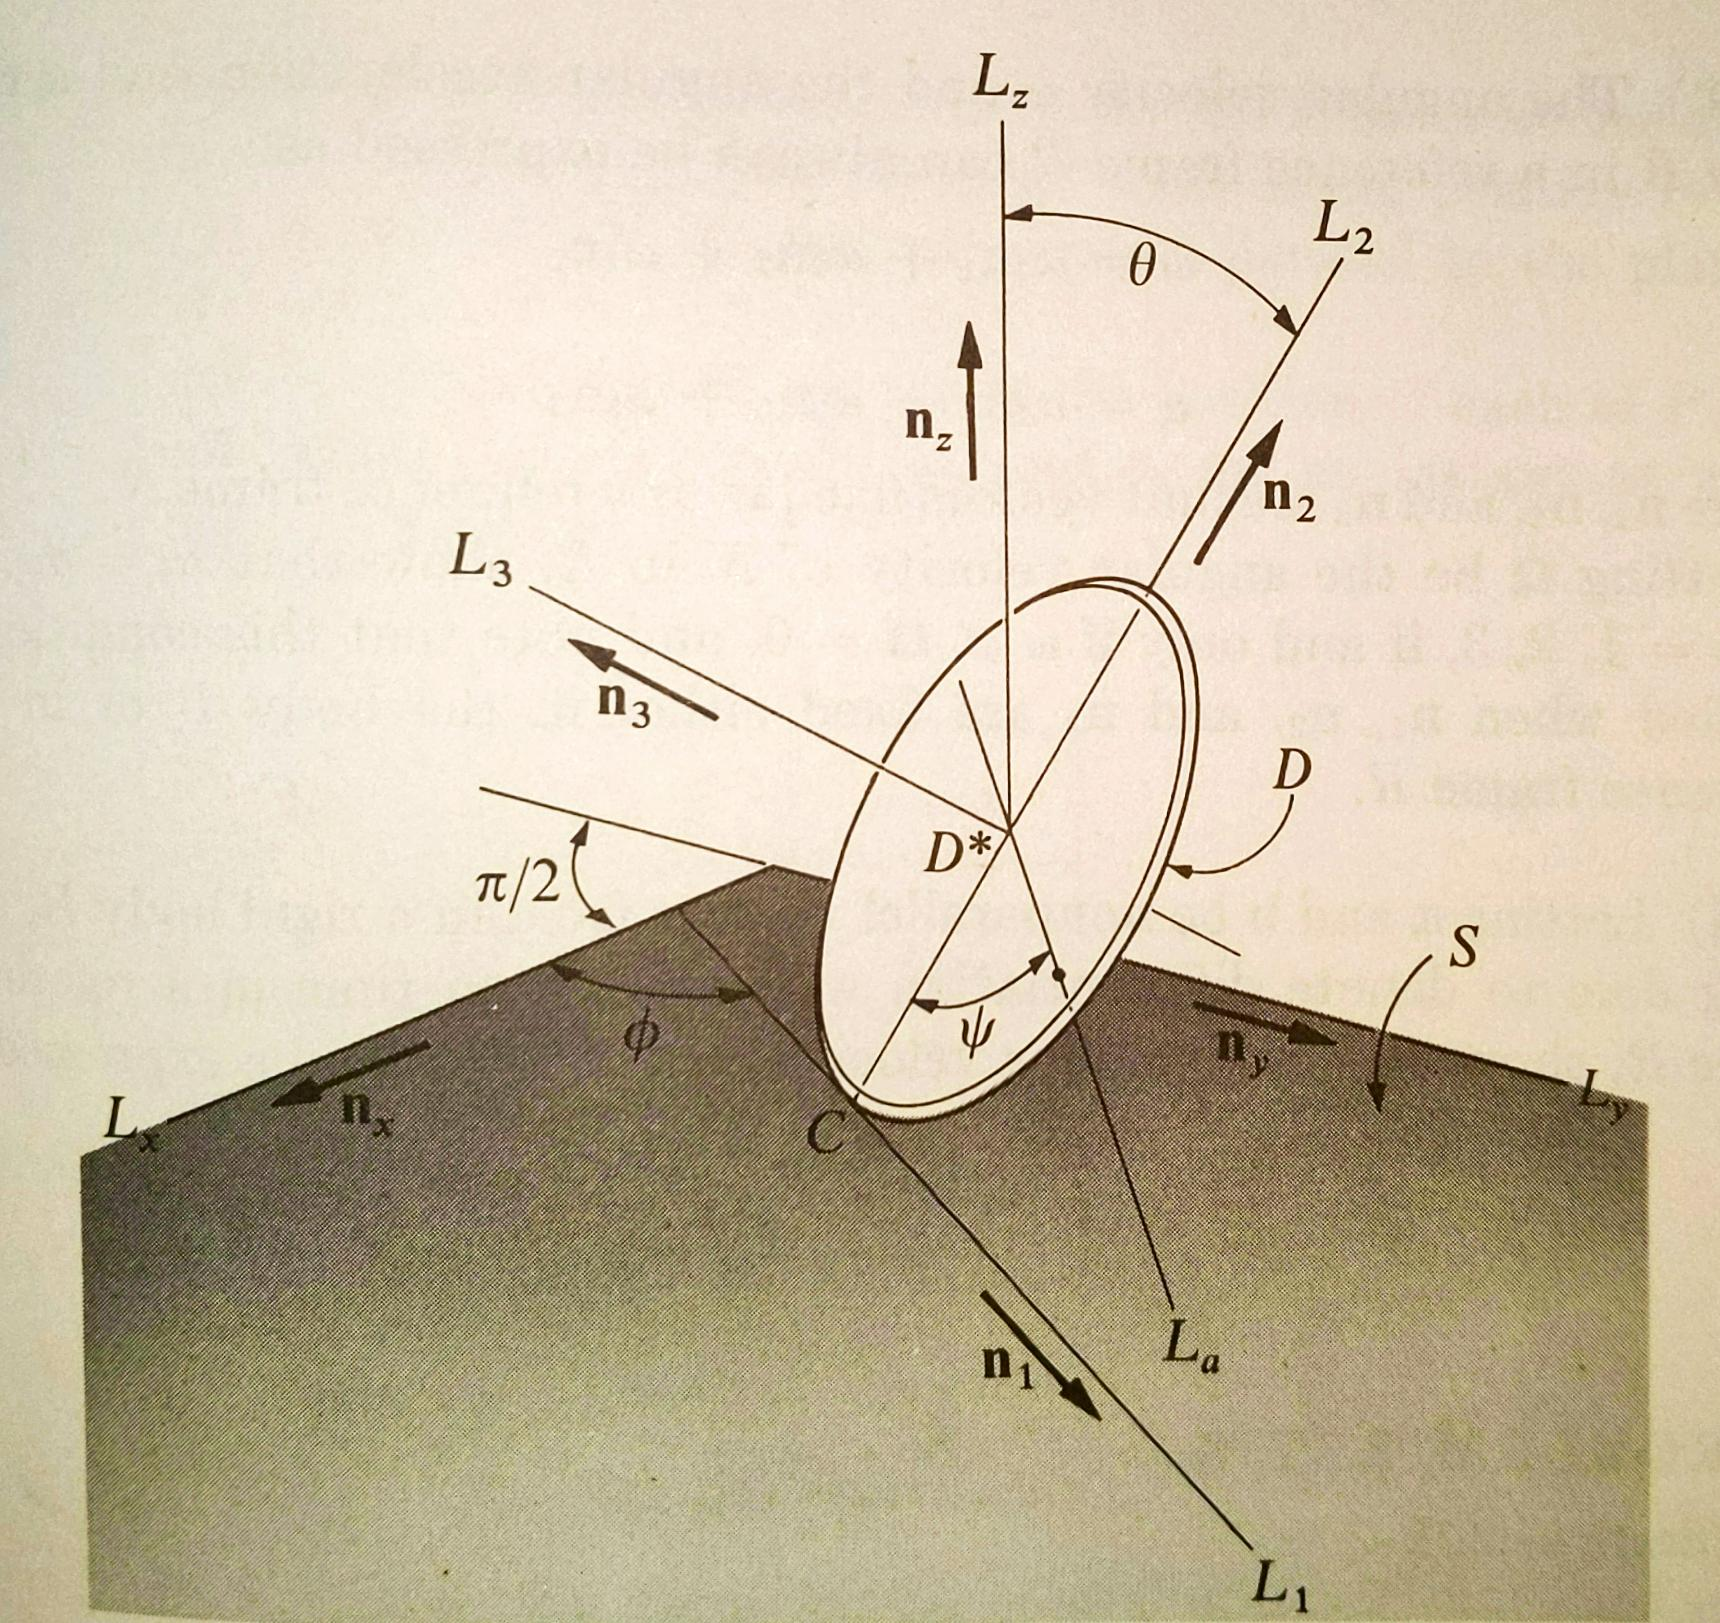
\includegraphics[width=0.7\textwidth, height=0.5\textwidth]{./figs/ProbSet_2/2_g.jpg}
    \caption{}
    \label{2_g}
\end{figure}
The transformation between the two coordinates $\pmb n_1, \pmb n_2, \pmb n_3$ and $\pmb n_x, \pmb n_y, \pmb n_z$ can be written as:
\begin{align*}
    \bm{\pmb n_1 \\ \pmb n_2 \\ \pmb n_3} &= \underbrace{R_1(90 - \theta) R_3(\phi)}_{R} \bm{\pmb n_x \\ \pmb n_y \\ \pmb n_z}\\
    R_1(90 - \theta) &= \bm{1 & 0 & 0 \\
                            0 & \cos (90-\theta) & \sin (90 - \theta) \\
                            0 &-\sin (90 - \theta) & \cos (90 - \theta)}
                      = \bm{1 & 0 & 0\\
                            0 & \sin \theta & \cos \theta \\
                            0 & -\cos \theta & \sin \theta} \\
    R_3(\phi) &= \bm{\cos \phi & \sin \phi & 0\\
                    -\sin \phi & \cos \phi & 0\\
                    0 & 0 & 1}\\
    R &=\bm{1 & 0 & 0\\
            0 & \sin \theta & \cos \theta \\
            0 & -\cos \theta & \sin \theta}
        \bm{\cos \phi & \sin \phi & 0\\
           -\sin \phi & \cos \phi & 0\\
            0 & 0 & 1}
    %==
        = \bm{\cos \phi & \sin \phi & 0\\
              -\sin \theta \sin \phi & \sin \theta \cos \phi & \cos \theta\\
              \cos \theta \sin \phi & -\cos \theta \cos \phi & \sin \theta}\\
    R^{-1} &=(R_1(90 - \theta) R_3(\phi))^{-1} = R_3^{-1} (\phi) R_1^{-1}(90 - \theta) = R_3^{T} (\phi) R_1^{T}(90 - \theta)\\
    &= \bm{\cos \phi & -\sin \phi & 0\\
          \sin \phi & \cos \phi & 0\\
           0 & 0 & 1}
        \bm{1 & 0 & 0\\
           0 & \sin \theta & -\cos \theta \\
           0 & \cos \theta & \sin \theta}
           %==
    = \bm{\cos \phi & - \sin \phi \sin \theta & \sin \phi \cos \theta \\
          \sin \phi & \cos \theta \cos \phi & - \cos \phi \cos \theta \\
          0         & \cos \theta           & \sin \theta }
\end{align*}

\begin{align*}
    \lx{^R}{\pmb \omega}^D &= - \dot \theta \pmb n_1 + \dot \phi \pmb n_z + \dot \psi \pmb n_3
    %===
    = - \dot \theta \pmb n_1 + \dot \phi \cos \theta \pmb n_2 + (\dot \phi \sin \theta + \dot \psi) \pmb n_3
\end{align*}

We have,
\begin{align*}
    \lx{^R}{\pmb \alpha}^B &= \lx{^R}{\frac{d\pmb \omega^B}{dt}}
    %==
    =\lx{^R}{\frac{d}{dt}}\left( - \dot \theta \pmb n_1 + \dot \phi \pmb n_z + \dot \psi \pmb n_3 \right)
    %==
    = - \ddot \theta \pmb n_1 - \dot \theta \dot{\pmb n}_1
       + \ddot \phi \pmb n_z + \dot \phi \dot{\pmb n}_z
       + \ddot \psi \pmb n_3 + \dot \psi \dot{\pmb n}_3
\end{align*}

also,
\begin{align*}
    \lx{^R}{\frac{d \pmb n_1}{dt}} &= \lx{^R}{\pmb \omega}^{L_1} \times \pmb n_1 = \dot \phi \pmb n_z \times \pmb n_1 = \dot \phi (\cos \theta \pmb n_2 + \sin \theta \pmb n_3) \times \pmb n_1\\
    &= \dot \phi (-\cos \theta \pmb n_3 +\sin \theta  \pmb n_2) \\
    %==
    \lx{^R}{\frac{d \pmb n_z}{dt}} &= 0 \qquad [\because \pmb n_z \text{ is fixed to the frame } R]
    \\
    %==
    \lx{^R}{\frac{d \pmb n_3}{dt}} &=  \lx{^R}{\pmb \omega}^{L_3} \times \pmb n_3
    = (\dot \phi \pmb n_z - \dot \theta \pmb n_1 ) \times \pmb n_3
    = (\dot \phi (\cos \theta \pmb n_2 + \sin \theta \pmb n_3) - \dot \theta \pmb n_1 ) \times \pmb n_3\\
    &= \dot \phi \cos \theta \pmb n_1 + \dot \theta \pmb n_2
\end{align*}

Substituting,
\begin{align*}
    \lx{^R}{\pmb \alpha}^B &=
       - \ddot \theta \pmb n_1 - \dot \theta (\dot \phi (-\cos \theta \pmb n_3 +\sin \theta  \pmb n_2) )
       + \ddot \phi (\cos \theta \pmb n_2 + \sin \theta \pmb n_3)
       + \ddot \psi \pmb n_3 + \dot \psi ( \dot \phi \cos \theta \pmb n_1 + \dot \theta \pmb n_2)\\
       &= \bm{
            \underbrace{
            -\ddot \theta + \dot \phi \dot \theta \cos \theta}_{\alpha_1} &
            \underbrace{
            -\dot \theta \dot \phi \sin \theta + \ddot \phi \cos \theta + \dot \psi \dot \theta }_{\alpha_2} &
            \underbrace{
            \dot \theta \dot \phi \cos \theta + \ddot \phi \sin \theta + \ddot \psi}_{\alpha_3}}
       \bm{\pmb n_1 \\ \pmb n_2 \\ \pmb n_3}\\
       %====
       &= \bm{\alpha_1 & \alpha_2 & \alpha_3} R
       \bm{\pmb n_x \\ \pmb n_y \\ \pmb n_z}
       %==
        = \bm{\alpha_1 & \alpha_2 & \alpha_3}
          \bm{\cos \phi & \sin \phi & 0\\
              -\sin \theta \sin \phi & \sin \theta \cos \phi & \cos \theta\\
              \cos \theta \sin \phi & -\cos \theta \cos \phi & \sin \theta}
            \bm{\pmb n_x \\ \pmb n_y \\ \pmb n_z}\\
        %==
        &= \bm{
            \alpha _1 \cos \phi - \alpha_2 \sin \theta \sin \phi + \alpha_3 \cos \theta \cos \phi &(=\alpha_x) \\
            \alpha_1 \sin \phi + \alpha_2 \sin \theta \cos \phi - \alpha_3 \cos \theta \cos \phi & (= \alpha_y)\\
            \alpha_2 \cos \theta + \alpha_3 \sin \theta & (=\alpha_z)}^T
        \bm{\pmb n_x \\ \pmb n_y \\ \pmb n_z}
\end{align*}

alternately,
\begin{align*}
    \lx{^R}{\pmb \omega}^D &= - \dot \theta \pmb n_1 + \dot \phi \pmb n_z + \dot \psi \pmb n_3\\
    %===
    &=-\dot \theta (\cos \phi \pmb n_x + \sin \phi \pmb n_y) + \dot \phi \pmb n_z + \dot \psi (\cos \theta \sin \phi \pmb n_x  -\cos \theta \cos \phi \pmb n_y  + \sin \theta \pmb n_z)\\
    %===
    &=\bm{-\dot \theta \cos \phi + \dot \psi \cos \theta \sin \phi &
         -\dot \theta \sin \phi - \dot \psi \cos \theta \cos \phi &
         \dot \phi + \dot \psi \sin \theta }
        \bm{\pmb n_x \\ \pmb n_y \\ \pmb n_z}
\end{align*}

Thus,
\begin{align*}
     \lx{^R}{\pmb \alpha}^B &= \lx{^R}{\frac{d\pmb \omega^B}{dt}}
     = \lx{^R}{\frac{d}{dt}} \left(\bm{-\dot \theta \cos \phi + \dot \psi \cos \theta \sin \phi &
         -\dot \theta \sin \phi - \dot \psi \cos \theta \cos \phi &
         \dot \phi + \dot \psi \sin \theta }
    \right) \bm{\pmb n_x \\ \pmb n_y \\ \pmb n_z}\\
    %==
    &=\bm{
        -\ddot \theta \cos \phi + \ddot \psi \cos \theta sin \phi + \dot \theta \dot \phi \sin \phi + \dot \psi \dot \phi \cos \theta \cos \phi - \dot \psi \dot \theta \cos \theta \sin \phi & (= \alpha_x)\\
        %==
        -\ddot \theta \sin \phi - \ddot \psi \cos \theta \cos \phi - \dot \theta \dot \phi \cos \phi + \dot \psi \dot \theta \sin \theta \cos \phi + \dot \psi \dot \phi \cos \theta \sin \phi & (= \alpha_y)\\
        %==
        \ddot \phi + \ddot \psi \sin \theta + \dot \psi \dot \theta \cos \theta & (=\alpha_z)
    }^T
    \bm{\pmb n_x \\ \pmb n_y \\ \pmb n_z}\\
\end{align*}

\itbf{Note:}
\begin{itemize}
    \item We can not just take $d \pmb n_z/dt$ as $\omega \times \pmb n_z$ in $\pmb n_1, \pmb n_2, \pmb n_3$ coordinates as $\pmb n_z$ is not rigidly fixed to the coordinates. This is only possible when $\pmb n_z$ does't change with time in $\pmb n_1, \pmb n_2, \pmb n_3$ frame. But once, the differentiation is done, one vector in $\pmb n_1, \pmb n_2, \pmb n_3$ frame can be written in $\pmb n_x, \pmb n_y, \pmb n_z$ frame using transformation matrices as they are instantaneous.

    \item Thus the rotation transformation can be used after differentiation as well.
\end{itemize}
